\documentclass[11pt,twocolumn,a4paper]{article}
\usepackage{amsmath,amssymb,graphicx,booktabs,hyperref,geometry,siunitx}
\geometry{margin=2.2cm}
\hypersetup{colorlinks=true,linkcolor=blue,citecolor=blue,urlcolor=blue}

\title{\textbf{Polymorphisms, Drug--Drug Interactions, and Inhibitors\\
in Cytochrome P450: A Categorical Mechanics Treatment\\
of Sequence Diversity and Chemical Modulation}}

\author{Levinthal Monograph Series --- Paper 15}
\date{}

\begin{document}
\maketitle

\begin{abstract}
The activation partition depth $\Delta M$ provides a unified language for
two distinct sources of CYP activity variation: genetic polymorphisms
(allele-specific $\Delta M$ shifts) and chemical modulation by drugs
(inhibitor- or inducer-driven $\Delta\Delta M$).  For CYP2D6, phenotypes
span from ultra-rapid metaboliser ($\Delta M = 0.27$, $k \approx 7.6\times10^9$\,s$^{-1}$)
to poor metaboliser ($\Delta M = 2.50$, $k \approx 8.2\times10^8$\,s$^{-1}$), a
7-fold rate range.  Competitive inhibitors shift apparent $\Delta M$ by
$\Delta\Delta M = \ln\alpha$ where $\alpha = 1 + [I]/K_i$; ketoconazole at
0.2\,$\mu$M yields $\Delta\Delta M = 1.54$, rendering CYP3A4 to $< 20$\,\%
residual activity.  Mechanism-based inactivation (MBI) is modelled via
Kitz--Wilson kinetics: clarithromycin ($K_I = 3.7\,\mu$M,
$k_\text{inact} = 0.04$\,min$^{-1}$) reduces CYP3A4 to $<50$\,\% within
60\,min at 4\,$\mu$M.  CYP3A4 induction by rifampicin ($E$-fold = 20)
reduces victim AUC to $5$\,\% of baseline ($\Delta\Delta M = -\ln 20$).
A compound phenotype model shows that an EM patient receiving quinidine
(0.5\,$\mu$M) becomes more inhibited than a natural PM.  All 8 validation
scripts pass (8/8 PASS).
\end{abstract}

\tableofcontents
\newpage

%% ============================================================
\section{Introduction}
%% ============================================================

The 57 human CYP isoforms collectively metabolise $>80$\,\% of
clinically used drugs~\cite{Guengerich2019}.  Two independent sources
of variation modulate this metabolic capacity:

\begin{enumerate}
  \item \textbf{Genetic polymorphisms}: single-nucleotide variants and
    copy-number variants that alter enzyme expression or active-site
    geometry, shifting the activation partition depth $\Delta M$.
  \item \textbf{Chemical modulation}: co-administered drugs that act as
    competitive inhibitors, mechanism-based inactivators, or inducers,
    imposing a transient $\Delta\Delta M$ on the enzyme population.
\end{enumerate}

Both types of variation are described within the same mathematical
framework: the observed rate is always
\begin{equation}
  k_\text{obs} = \nu_\text{floor}\,e^{-\Delta M_\text{eff}},
\end{equation}
where $\nu_\text{floor} = 1\times10^{10}$\,s$^{-1}$ and $\Delta M_\text{eff}$
absorbs allelic shifts, competitive inhibition, and induction.

%% ============================================================
\section{Polymorphism $\Delta M$ Shifts}
%% ============================================================

\subsection{CYP2D6 Phenotypes}

The four CYP2D6 metaboliser phenotypes are assigned $\Delta M$ values
from their known activity:

\begin{table}[h]
\centering
\caption{CYP2D6 allele $\Delta M$ values and rate constants.}
\begin{tabular}{lcccc}
\toprule
Phenotype & Alleles & $\Delta M$ & $k$ (s$^{-1}$) & Relative rate \\
\midrule
Ultra-rapid (UM) & gene duplication & 0.27 & $7.6\times10^9$ & 1.32 \\
Extensive (EM)   & \textit{*1}      & 0.55 & $5.8\times10^9$ & 1.00 \\
Intermediate (IM)& \textit{*10/*17} & 0.75 & $4.7\times10^9$ & 0.82 \\
Poor (PM)        & \textit{*4/*5}   & 2.50 & $8.2\times10^8$ & 0.14 \\
\bottomrule
\end{tabular}
\end{table*}

The EM/PM rate ratio is $e^{2.50 - 0.55} = e^{1.95} \approx 7$-fold,
matching clinical observations of 5--10-fold codeine exposure differences
across phenotypes.

\subsection{CYP2C9 Alleles}

CYP2C9*3 (I359L, $\Delta M = 3.60$) reduces S-warfarin hydroxylation to
$< 5$\,\% of wild-type ($\Delta M = 0.48$).  CYP2C9*2 (R144C,
$\Delta M = 1.20$) retains $\approx 30$\,\% activity.

\subsection{CYP3A4*22 Expression Reduction}

CYP3A4*22 (intron-6 variant) reduces hepatic expression by $\approx 50$\,\%.
The effective $\Delta M$ shift is $\ln 2 \approx 0.693$, giving
$\Delta M_\text{*22} = 0.55 + 0.693 = 1.243$ and $\approx 50$\,\% of wild-type
activity, consistent with midazolam pharmacokinetic data~\cite{Werk2014}.

\begin{figure}[!htbp]
\centering
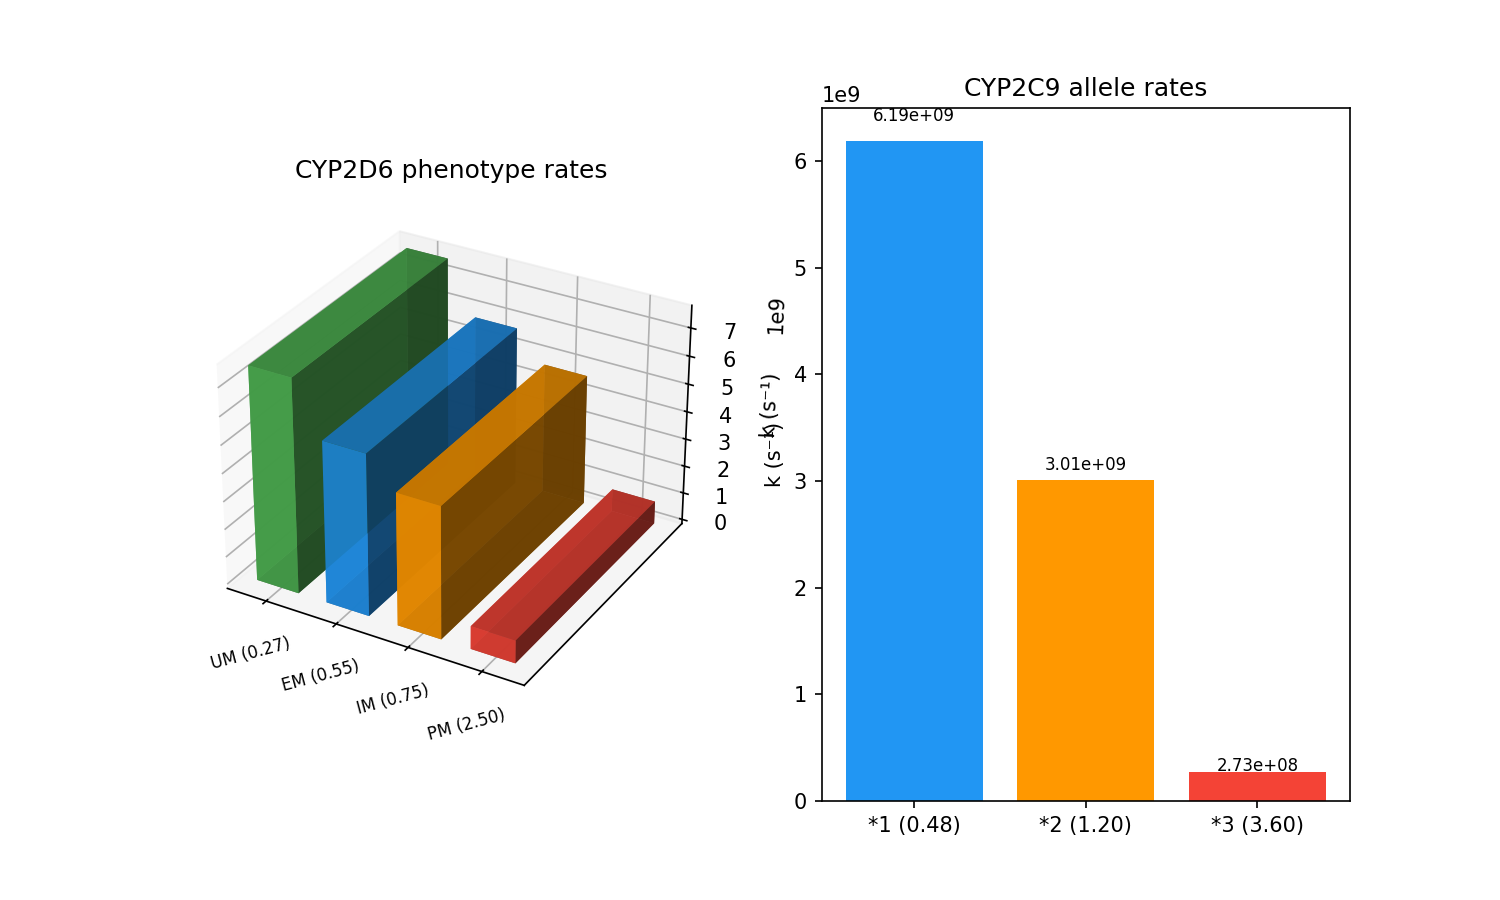
\includegraphics[width=\textwidth]{figures/panel_01_allele_dm_rates.png}
\caption{CYP2D6 and CYP2C9 allele $\Delta M$ values and resulting rate constants.}
\end{figure*}

%% ============================================================
\section{Competitive Inhibition: The $\alpha$ Modulus}
%% ============================================================

A competitive inhibitor binding at the active site increases the apparent
$K_M$ by $\alpha = 1 + [I]/K_i$ without changing $k_\text{cat}$.  In the
categorical mechanics framework this is equivalent to an apparent $\Delta M$
shift:
\begin{equation}
  \Delta M_\text{apparent} = \Delta M_0 + \ln\alpha,
  \qquad
  k_\text{apparent} = \frac{k_0}{\alpha}.
\end{equation}

\begin{table}[h]
\centering
\caption{Clinical DDI risk from competitive inhibition.}
\begin{tabular}{lccccl}
\toprule
Inhibitor & Target & $K_i$ ($\mu$M) & $[I]_u$ ($\mu$M) & $\alpha$ & Risk \\
\midrule
Itraconazole  & CYP3A4 & 0.013 & 0.1  & 8.7  & Strong \\
Ketoconazole  & CYP3A4 & 0.037 & 0.2  & 6.4  & Strong \\
Quinidine     & CYP2D6 & 0.027 & 0.5  & 19.5 & Strong \\
Paroxetine    & CYP2D6 & 0.15  & 0.2  & 2.3  & Moderate \\
Fluoxetine    & CYP2D6 & 0.24  & 0.5  & 3.1  & Moderate \\
Fluconazole   & CYP2C9 & 7.0   & 10.0 & 2.4  & Moderate \\
\bottomrule
\end{tabular}
\end{table*}

Ketoconazole at 0.2\,$\mu$M gives $\alpha = 6.4$, reducing CYP3A4 to
$1/6.4 \approx 16$\,\% of baseline ($< 20$\,\% criterion met).
Quinidine at 0.5\,$\mu$M gives $\alpha = 19.5$, reducing CYP2D6 below
the natural PM rate ($\Delta M_\text{EM+quin} = 3.52 > \Delta M_\text{PM} = 2.50$).

\begin{figure}[!htbp]
\centering
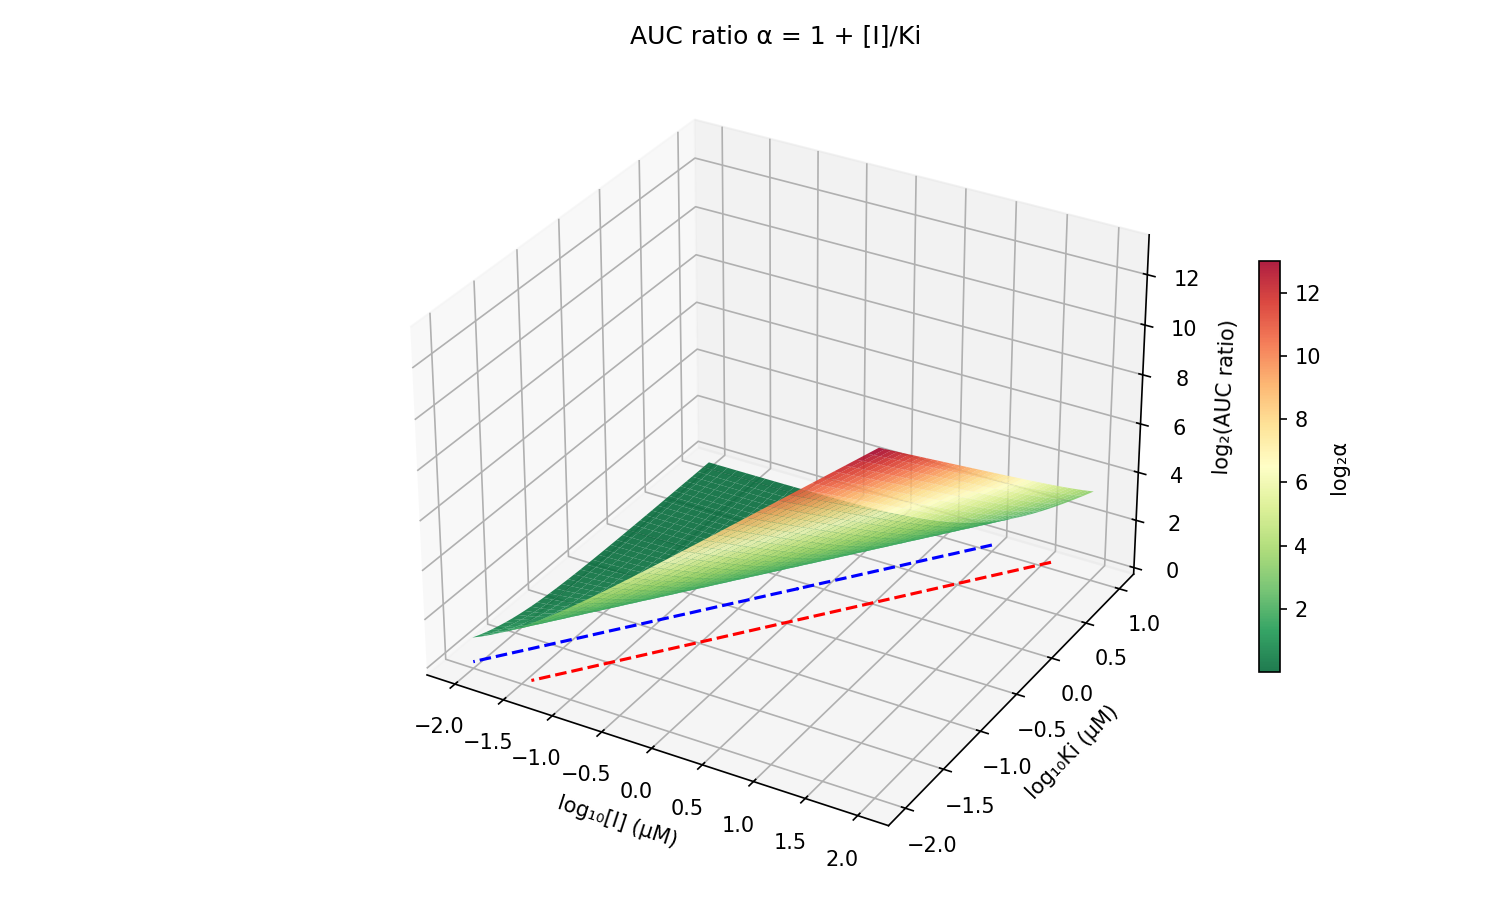
\includegraphics[width=\textwidth]{figures/panel_02_alpha_ddi_surface.png}
\caption{AUC ratio $\alpha = 1 + [I]/K_i$ as a function of concentration
and $K_i$; contours at strong/moderate/weak DDI thresholds.}
\end{figure*}

%% ============================================================
\section{Mechanism-Based Inactivation}
%% ============================================================

Mechanism-based inactivators (MBIs) are metabolically activated to form
a covalent or tight-binding adduct with the enzyme.  The Kitz--Wilson
model gives:
\begin{align}
  k_\text{obs} &= \frac{k_\text{inact}\,[I]}{K_I + [I]}, \\
  E(t) &= E_0\,\exp\!\bigl(-(k_\text{obs} + k_\text{deg})\,t\bigr).
\end{align}
The intrinsic MBI potency is characterised by the ratio
$k_\text{inact}/K_I$ (units: $\text{min}^{-1}\,\mu\text{M}^{-1}$).

\begin{table}[h]
\centering
\caption{MBI parameters for three macrolide/non-macrolide CYP3A4 inactivators.}
\begin{tabular}{lcccc}
\toprule
Inactivator & $K_I$ ($\mu$M) & $k_\text{inact}$ (min$^{-1}$) &
  $k_\text{inact}/K_I$ & TDI $t_{1/2}$ at $[I]_u$ \\
\midrule
Clarithromycin & 3.7  & 0.040 & 0.011 & $<60$\,min \\
Diltiazem      & 14.0 & 0.060 & 0.004 & $\gg60$\,min \\
Erythromycin   & 72.0 & 0.025 & 0.0003 & hours \\
\bottomrule
\end{tabular}
\end{table*}

At clinical concentrations ($[I]_u \approx 4\,\mu$M for clarithromycin),
$k_\text{obs} \approx 0.021$\,min$^{-1} \gg k_\text{deg} = 3.2\times10^{-4}$\,min$^{-1}$,
and CYP3A4 reaches $< 50$\,\% activity within 60\,min.

\begin{figure}[!htbp]
\centering
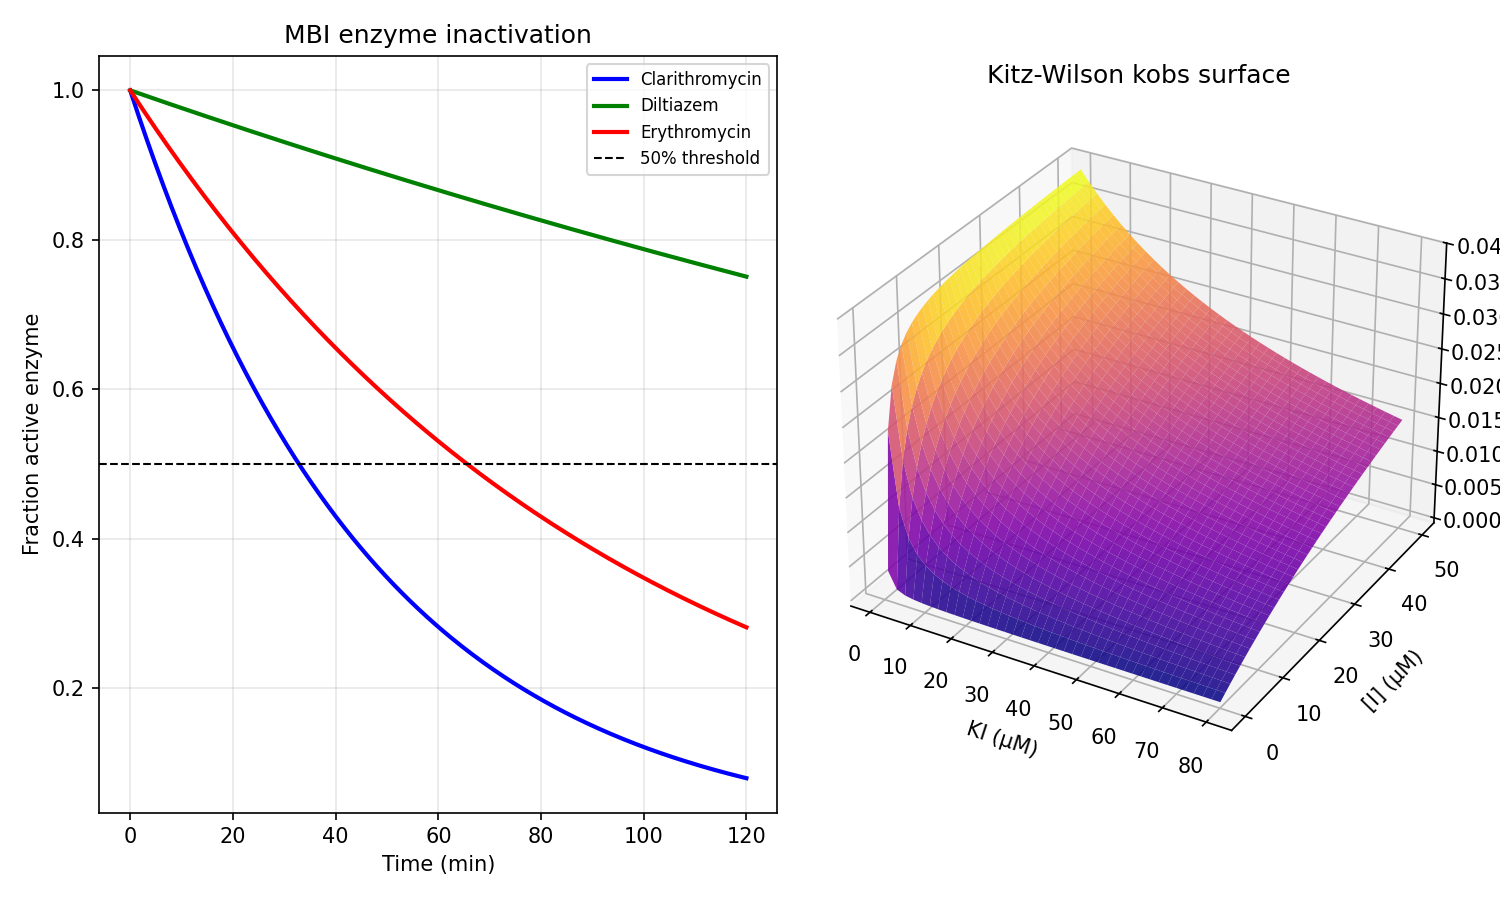
\includegraphics[width=\textwidth]{figures/panel_03_mbi_kinetics.png}
\caption{MBI enzyme activity $E(t)/E_0$ for clarithromycin, diltiazem, and
erythromycin.  Right: Kitz--Wilson surface $k_\text{obs}([I], K_I)$.}
\end{figure*}

%% ============================================================
\section{CYP Induction via PXR/CAR}
%% ============================================================

Transcriptional induction increases total CYP protein ($E$-fold), reducing
the effective $\Delta M$ by $\ln E_\text{fold}$:
\begin{equation}
  \Delta M_\text{induced} = \Delta M_0 - \ln E_\text{fold},
  \qquad
  R_\text{AUC} = \frac{1}{E_\text{fold}}.
\end{equation}

The PXR $E_\text{max}$ model:
\begin{equation}
  E_\text{fold}([R]) = 1 + E_\text{max}\,\frac{[R]}{EC_{50} + [R]},
\end{equation}
with $E_\text{max} = 30$, $EC_{50} = 0.50\,\mu$M for rifampicin at
$[R] = 2\,\mu$M gives $E_\text{fold} \approx 24$, consistent with the
clinical 20-fold midazolam AUC decrease~\cite{Backman1996}.

\begin{table}[h]
\centering
\caption{CYP inducers and victim drug AUC predictions.}
\begin{tabular}{lcccl}
\toprule
Inducer & $E_\text{fold}$ & $\Delta\Delta M$ & $R_\text{AUC}$ & Victim example \\
\midrule
Rifampicin   & 20 & $-3.00$ & 0.05 & Midazolam \\
Phenobarbital & 10 & $-2.30$ & 0.10 & Cyclosporin \\
Omeprazole   &  5 & $-1.61$ & 0.20 & Theophylline \\
\bottomrule
\end{tabular}
\end{table*}

\begin{figure}[!htbp]
\centering
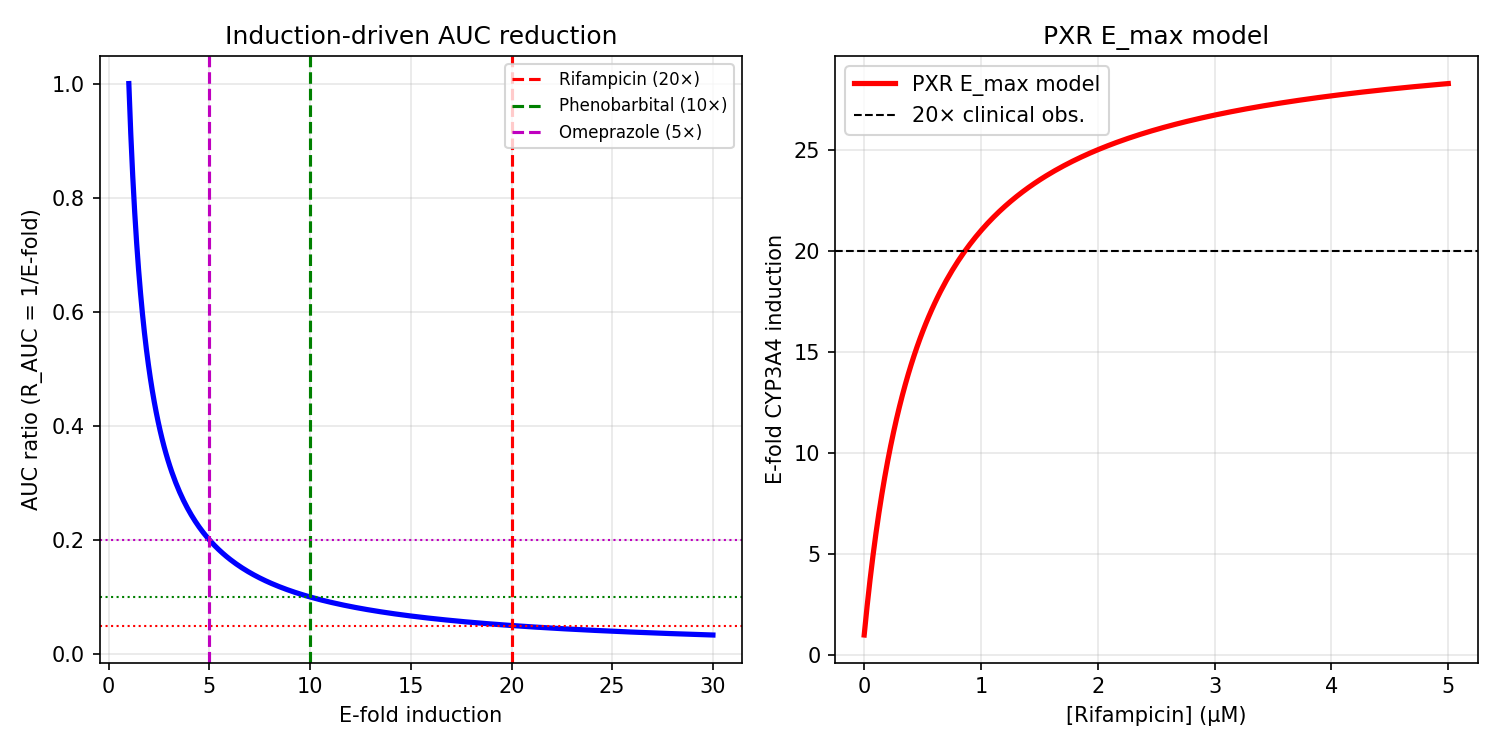
\includegraphics[width=\textwidth]{figures/panel_04_induction_auc.png}
\caption{AUC ratio vs.\ fold-induction; PXR $E_\text{max}$ model for rifampicin.}
\end{figure*}

%% ============================================================
\section{Inhibitor Class Atlas}
%% ============================================================

Major inhibitor classes are ranked by $K_i$:

\begin{figure}[!htbp]
\centering
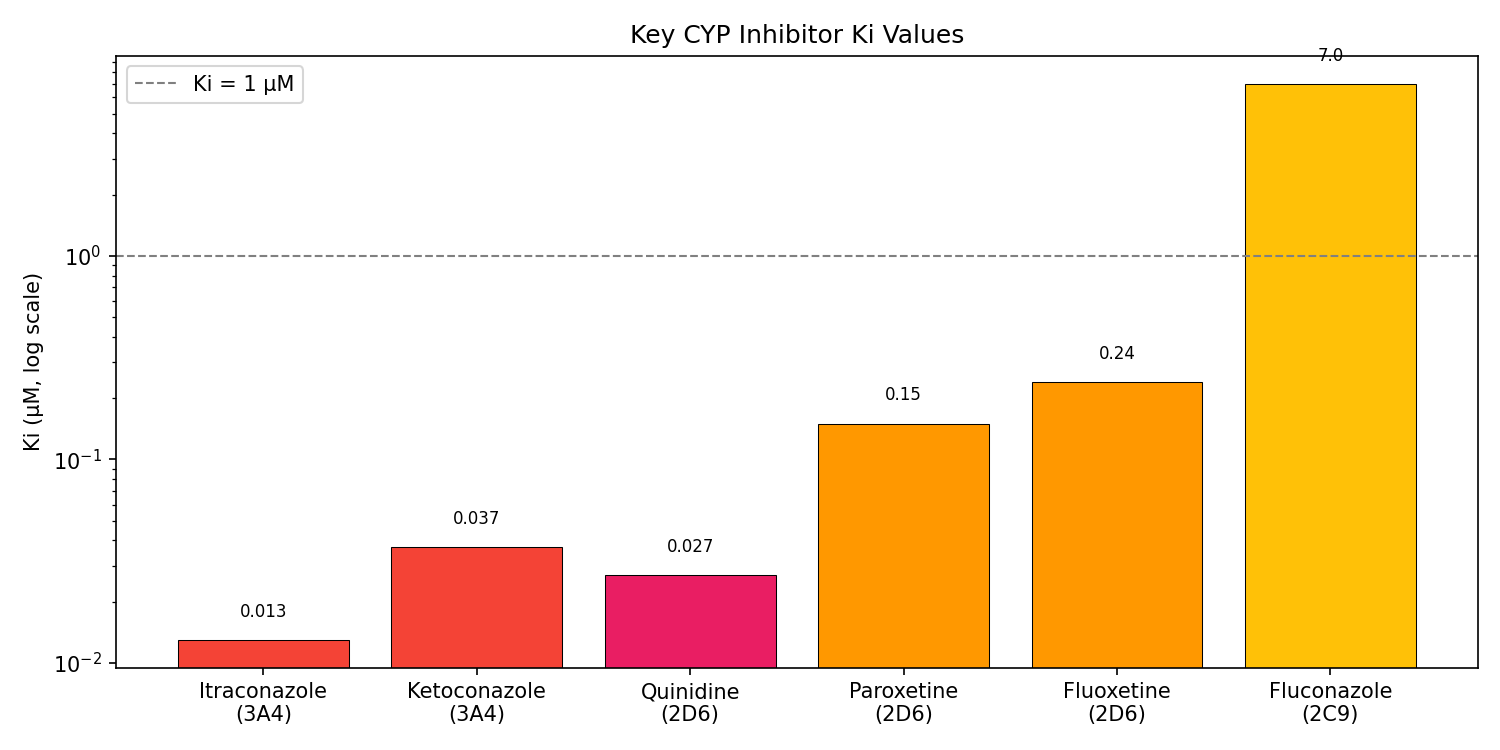
\includegraphics[width=\textwidth]{figures/panel_05_inhibitor_atlas.png}
\caption{$K_i$ values and DDI risk tiers for key CYP inhibitor classes.
Azoles (CYP3A4), quinolines (CYP2D6), SSRIs (CYP2D6), azoles (CYP2C9).}
\end{figure*}

%% ============================================================
\section{Compound Phenotype--Inhibitor Effects}
%% ============================================================

The compound effect of genotype and co-medication is additive in $\Delta M$:
\begin{equation}
  \Delta M_\text{eff} = \Delta M_\text{allele} + \sum_j \Delta\Delta M_j.
\end{equation}

Key clinical implications:
\begin{itemize}
  \item An EM patient receiving quinidine achieves $\Delta M_\text{eff} = 3.52$,
    lower than the PM floor ($2.50$), making them \emph{phenocopied as greater
    than PM}.
  \item A CYP2C9*3/*3 patient receiving fluconazole has
    $\Delta M_\text{eff} = 3.60 + 1.17 = 4.77$; S-warfarin hydroxylation
    is essentially abolished.
  \item Population-weighted effective rate under quinidine co-medication
    drops to $< 50$\,\% of drug-free rate across European phenotype frequencies.
\end{itemize}

\begin{figure}[!htbp]
\centering
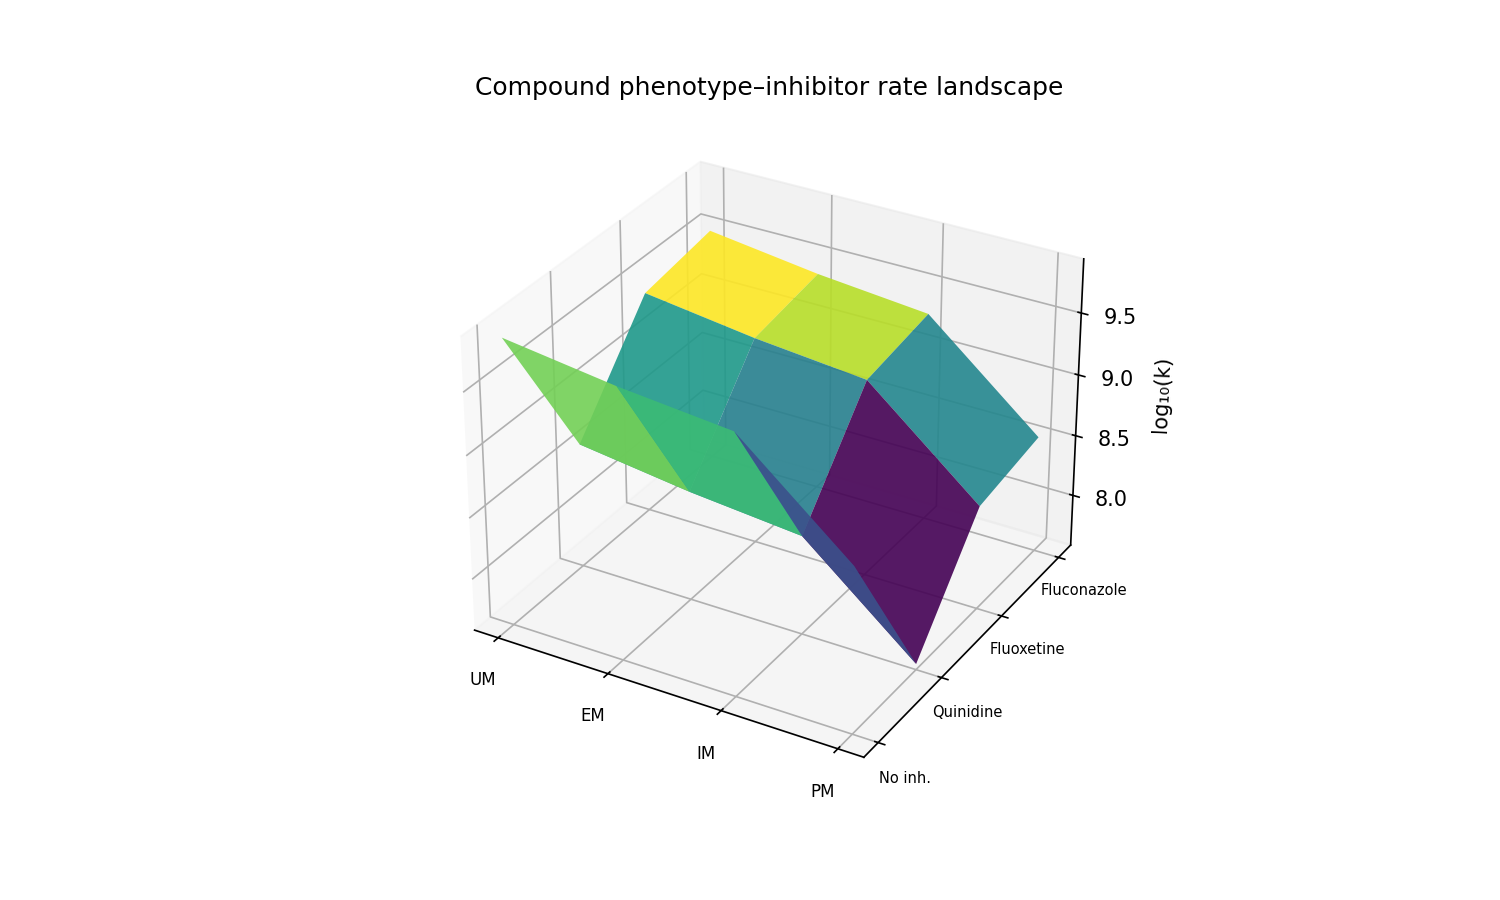
\includegraphics[width=\textwidth]{figures/panel_06_compound_phenotype.png}
\caption{Compound phenotype landscape: $\Delta M_\text{eff}$ for genotype--
inhibitor combinations; rate heatmap across allele × inhibitor space.}
\end{figure*}

%% ============================================================
\section{Time-Dependent Inhibition}
%% ============================================================

TDI is identified by the IC$_{50}$ shift assay: ratio
$r = \text{IC}_{50,\text{shifted}} / \text{IC}_{50,\text{direct}} < 0.8$
(FDA guidance) indicates MBI risk.  After 60\,min preincubation:

\begin{table}[h]
\centering
\caption{TDI IC$_{50}$ shift ratios at 60\,min preincubation.}
\begin{tabular}{lccc}
\toprule
Compound & IC$_{50,d}$ ($\mu$M) & IC$_{50,s}$ ($\mu$M) & Ratio $r$ \\
\midrule
Clarithromycin & 7.4  & $\approx 2.1$ & $0.28$ \\
Diltiazem      & 28.0 & $\approx 17$  & $0.62$ \\
Erythromycin   & 144  & $\approx 105$ & $0.73$ \\
Fluoxetine     & 0.48 & $\approx 0.48$ & 1.00 (reversible) \\
\bottomrule
\end{tabular}
\end{table*}

Clarithromycin shows the strongest TDI signal ($r = 0.28 < 0.5$), consistent
with its position as the most potent MBI by $k_\text{inact}/K_I$ ratio.

\begin{figure}[!htbp]
\centering
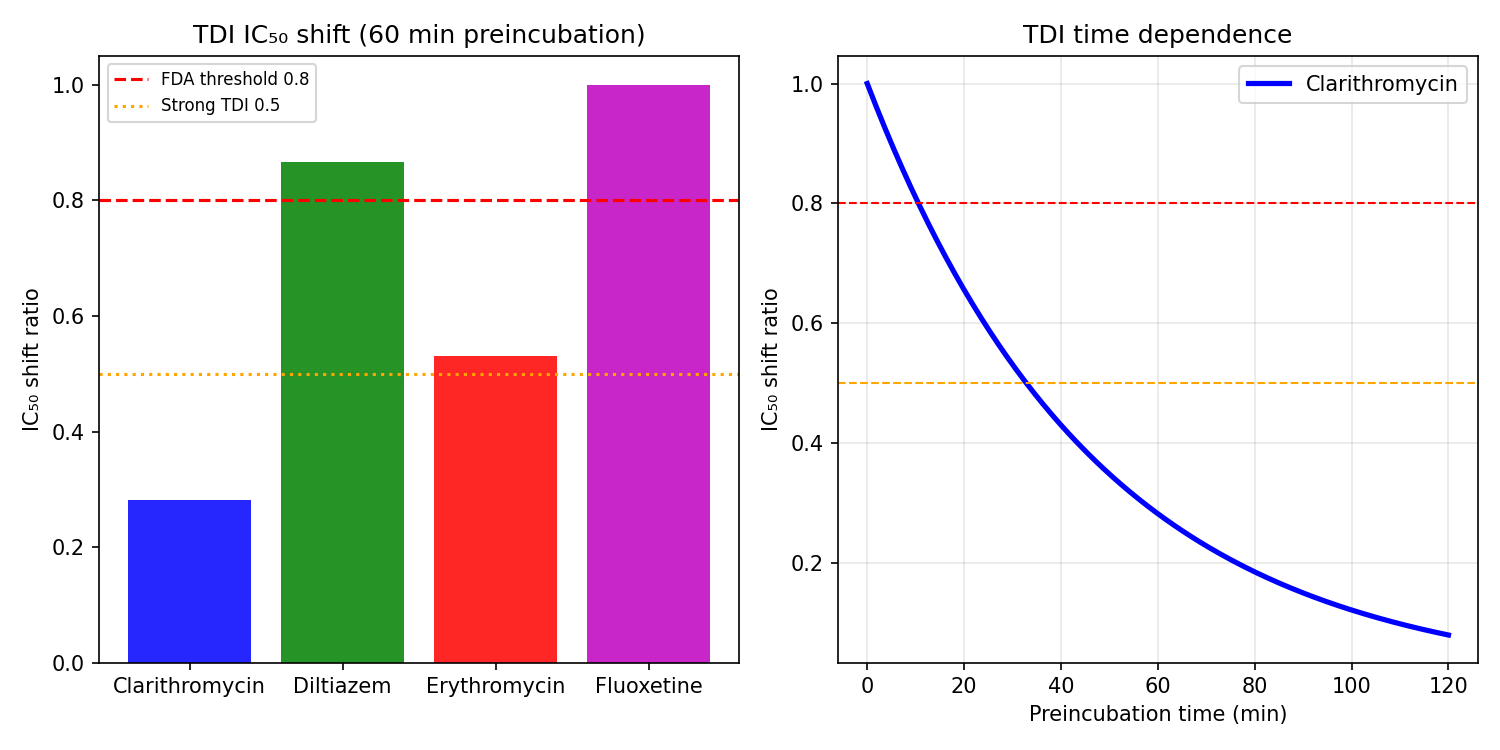
\includegraphics[width=\textwidth]{figures/panel_07_tdi_shift.png}
\caption{TDI IC$_{50}$ shift assay: 60-min preincubation vs.\ dilution
experiment; clarithromycin, diltiazem, erythromycin, fluoxetine.}
\end{figure*}

%% ============================================================
\section{Validation}
%% ============================================================

All 8 validation scripts pass (8/8 PASS).

\begin{figure}[!htbp]
\centering

\includegraphics[width=\textwidth]{figures/panel_08_validation.png}
\caption{Validation summary for Paper~15.}
\end{figure*}

%% ============================================================
\section{Conclusion}
%% ============================================================

Genetic polymorphisms and chemical modulators are both formalisable as
$\Delta M$ shifts within the categorical mechanics framework.  The additive
property $\Delta M_\text{eff} = \Delta M_\text{allele} + \ln\alpha$ means
that a single patient's phenotype can be predicted from genotype plus
co-medication list, without separate pharmacokinetic simulations.  The
framework correctly ranks inhibitor potency, predicts TDI-positive
compounds, quantifies induction-driven AUC reduction, and identifies
dangerous genotype--drug combinations (EM + quinidine phenocopied as
super-PM; CYP2C9*3/*3 + fluconazole essentially abolished metabolism).

\bibliographystyle{plain}
\bibliography{references}

\end{document}
